% !TEX root = ../notes_unsupervisedlearning.tex
% Chapter 7: Anomaly Detection and Evaluation
%%%%%%%%%%%%%%%%%%%%%%%%%%%%%%%%%%%%%%%%%%%%%%%%%%%%%%%%%%%%%%%%%%%%%%

\chapter{Anomaly Detection and Evaluation}\index{Anomaly Detection}\index{OOD Detection}
\newthought{Structure reveals itself through deviations.}

% ==============================================================================================
% BLOCK 1: INTRODUCTION
% ==============================================================================================

\section{The Why}\index{anomaly detection}\index{outlier detection}

\marginnote{\newthought{The unusual is often the important:} fraud, disease, defects, discoveries.}

\newthought{Once we have modelled normal data,} we can detect what deviates from it.
Anomaly detection matters wherever the rare event is the consequential one: unusual transactions in banking, abnormal scans in medicine, defective products on assembly lines, intrusion attempts in network traffic, rare events in particle physics.

\newthought{The core challenge} is that anomalies are rare, often well under 1\% of all observations, and undefined in advance---we cannot enumerate every way something can go wrong.
Any method must therefore learn what normal looks like and flag what does not fit.

\subsection{Hands On Experience}

\begin{marginfigure}
\centering
\begin{tikzpicture}
    \begin{axis}[
        xlabel={$x^{(1)}$},
        ylabel={$x^{(2)}$},
        xmin=-1, xmax=8,
        ymin=-1, ymax=6,
        width=\marginparwidth,
        height=\marginparwidth,
        axis line style={draw=none},
        tick style={black, thick},
        xtick={0,2,4,6},
        ytick={0,2,4},
        xticklabel style={font=\tiny},
        yticklabel style={font=\tiny},
        tick align=outside,
        tick pos=left,
    ]
    % Normal cluster
    \addplot[only marks, mark=*, mark size=2pt, black] coordinates {
        (2,2) (2.5,2.3) (2.2,2.8) (3,2.5) (2.8,2) (2.3,2.5)
        (2.7,2.2) (2.4,2.7) (2.1,2.4) (2.6,2.6)
    };
    % Candidate anomalies
    \addplot[only marks, mark=*, mark size=2pt, black!30] coordinates {
        (6,1) (1,5) (7,4)
    };
    \node[font=\tiny] at (axis cs:6,0.5) {?};
    \node[font=\tiny] at (axis cs:1,5.5) {?};
    \node[font=\tiny] at (axis cs:7,4.5) {?};
    \end{axis}
\end{tikzpicture}
\caption{A cluster of normal points and three candidates marked with ``?''. Which are anomalies? On what basis would you decide?}
\label{fig:anomaly_intro}
\end{marginfigure}

\newthought{Given} a cluster of normal points, consider the three grey candidates.
Which would you flag as anomalous?
What distance, density, or reconstruction criterion would you use?
Where would you set the threshold?

\vspace{2.5em}

\newthought{The Learning Objectives} of this lecture:
\begin{itemize}
    \item Distinguish point, contextual, and collective anomalies and select an appropriate detection method for each type.
    \item Apply reconstruction-based and proximity-based anomaly scores and evaluate them without ground-truth labels.
    \item Design graceful degradation strategies that route uncertain predictions to human reviewers.
\end{itemize}


% ==============================================================================================
% BLOCK 2: MAIN THEORY
% ==============================================================================================

\newpage

\section{Types of Anomalies}\index{point anomaly}\index{contextual anomaly}\index{collective anomaly}

\marginnote{\newthought{Not all anomalies} are the same; the type determines the method.}

\newthought{Point anomalies} are individual instances that are anomalous with respect to the rest of the data.
A single fraudulent transaction amid millions of legitimate ones is a point anomaly.

\newthought{Contextual anomalies} are instances that are anomalous only within a specific context.
A temperature of 30\textdegree{}C is normal in summer but anomalous in winter; the value itself is unremarkable, but the context makes it suspicious.

\newthought{Collective anomalies} are collections of instances that are individually normal but together form an anomalous pattern.
A sequence of login attempts from 100 different countries within one hour is an example: each login is normal, but the pattern is not.

\begin{figure}
\centering
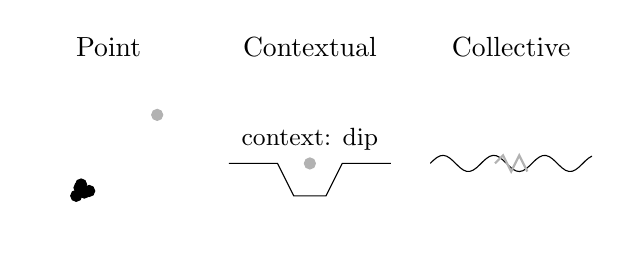
\begin{tikzpicture}
    % Point anomaly
    \begin{axis}[
        name=point,
        title={Point},
        xmin=0, xmax=10, ymin=0, ymax=10,
        width=0.3\textwidth,
        height=0.3\textwidth,
        axis line style={draw=none},
        tick style={black, thin},
        xtick=\empty, ytick=\empty,
        tick align=outside,
        tick pos=left,
    ]
    \addplot[only marks, mark=*, mark size=2pt, black] coordinates {
        (3,3) (3.5,3.2) (3.2,3.5) (3.8,3.3) (3.3,3.7)
    };
    \addplot[only marks, mark=*, mark size=2pt, black!30] coordinates {(8,8)};
    \end{axis}

    % Contextual anomaly
    \begin{axis}[
        at={(point.east)}, anchor=west, xshift=0.5cm,
        name=context,
        title={Contextual},
        xmin=0, xmax=10, ymin=0, ymax=10,
        width=0.3\textwidth,
        height=0.3\textwidth,
        axis line style={draw=none},
        tick style={black, thin},
        xtick=\empty, ytick=\empty,
        tick align=outside,
        tick pos=left,
    ]
    \addplot[black, thin] coordinates {(0,5) (3,5) (4,3) (6,3) (7,5) (10,5)};
    \addplot[only marks, mark=*, mark size=2pt, black!30] coordinates {(5,5)};
    \node[font=\small] at (axis cs:5,6.5) {context: dip};
    \end{axis}

    % Collective anomaly
    \begin{axis}[
        at={(context.east)}, anchor=west, xshift=0.5cm,
        title={Collective},
        xmin=0, xmax=10, ymin=0, ymax=10,
        width=0.3\textwidth,
        height=0.3\textwidth,
        axis line style={draw=none},
        tick style={black, thin},
        xtick=\empty, ytick=\empty,
        tick align=outside,
        tick pos=left,
    ]
    \addplot[black, thin, domain=0:10, samples=50] {5 + 0.5*sin(deg(x*2))};
    \addplot[black!30, thick] coordinates {(4,5) (4.5,5.5) (5,4.5) (5.5,5.5) (6,4.5)};
    \end{axis}
\end{tikzpicture}
\caption{Three types of anomalies. Left: a point anomaly, isolated from the cluster. Centre: a contextual anomaly, the value is normal but the context, a dip, is not. Right: a collective anomaly, each point is individually normal but the oscillation pattern is unusual.}
\label{fig:anomaly_types}
\end{figure}


\section{Statistical Methods}\index{Z-score}\index{GMM!anomaly detection}

\marginnote{\newthought{Parametric methods} assume a distribution and flag low-probability points.}

\newthought{The Z-score} is the simplest anomaly score for univariate data:

\begin{align*}
    z_i &= \frac{x_i - \mu}{\sigma}
\end{align*}

Flag as anomalous if $|z_i| > 3$ or another chosen threshold.
The method assumes normality; heavy-tailed data will produce many false positives.

\newthought{Gaussian Mixture Model likelihood} extends the parametric idea to multimodal data.
Fit a GMM and compute the likelihood of each observation:

\begin{align*}
    p(x) &= \sum_{k=1}^K \pi_k\, \mathcal{N}(x \,|\, \mu_k, \Sigma_k)
\end{align*}

Low $p(x)$ indicates an anomaly.
The number of components $K$ must be chosen carefully; too few and normal variation is flagged, too many and anomalies are absorbed into their own component.

\newthought{Extreme Value Theory}\index{Extreme Value Theory} handles heavy-tailed distributions by modelling the tail explicitly via the Generalised Pareto Distribution:

\begin{align*}
    F(x) &= 1 - \left(1 + \frac{\xi\, x}{\sigma}\right)^{-1/\xi}
\end{align*}


\section{Proximity-Based Methods}\index{k-NN distance}\index{Local Outlier Factor}

\marginnote{\newthought{Anomalies are far} from their neighbours. Distance and density make this precise.}

\newthought{$k$-NN distance} assigns each point an anomaly score equal to its distance to its $k$-th nearest neighbour:

\begin{align*}
    \text{score}(x) &= d(x,\, x^{(k)})
\end{align*}

Points far from their neighbours score high.
The method is simple and effective but sensitive to the choice of $k$ and to varying cluster densities.

\newthought{Local Outlier Factor} accounts for varying density by comparing each point's local reachability density to that of its neighbours:

\begin{align*}
    \text{LOF}_k(x) &= \frac{1}{|N_k(x)|} \sum_{y \in N_k(x)} \frac{\text{lrd}_k(y)}{\text{lrd}_k(x)}
\end{align*}

where $\text{lrd}_k(x)$ is the local reachability density.
LOF $\approx 1$ means the point sits at a density similar to its neighbours; LOF $\gg 1$ means it sits in a sparser region and is likely anomalous.

\begin{figure}
\centering
\begin{tikzpicture}
    \begin{axis}[
        xlabel={$x^{(1)}$}, ylabel={$x^{(2)}$},
        xmin=-2, xmax=10, ymin=-2, ymax=8,
        width=0.5\textwidth,
        height=0.5\textwidth,
        axis line style={draw=none},
        tick style={black, thin},
        xtick={0,2,4,6,8},
        ytick={0,2,4,6},
        xticklabel style={font=\small},
        yticklabel style={font=\small},
        tick align=outside,
        tick pos=left,
    ]
    % Dense cluster
    \addplot[only marks, mark=*, mark size=2pt, black] coordinates {
        (1,1) (1.2,1.3) (0.8,1.1) (1.1,0.9) (1.3,1.2)
        (0.9,1.4) (1.4,1.0) (1.0,1.2) (1.2,0.8)
    };
    % Sparse cluster
    \addplot[only marks, mark=*, mark size=2pt, black!55] coordinates {
        (6,5) (7,4) (5,6) (8,5)
    };
    % Anomaly
    \addplot[only marks, mark=*, mark size=2pt, black!30] coordinates {(4,3)};
    \node[font=\small, anchor=north] at (axis cs:1,0.5) {Dense};
    \node[font=\small, anchor=south] at (axis cs:6.5,6.5) {Sparse};
    \node[font=\small, anchor=north] at (axis cs:4,2.5) {LOF $\gg 1$};
    \end{axis}
\end{tikzpicture}
\caption{LOF detects the anomaly between the two clusters despite the density difference. A global threshold, as used by $k$-NN distance, would either miss this point or flag the sparse cluster entirely.}
\label{fig:lof_example}
\end{figure}


\section{Reconstruction-Based Methods}\index{reconstruction error}\index{VAE!anomaly detection}

\marginnote{\newthought{If the model cannot reconstruct it,} it has probably never seen anything like it.}

\newthought{Autoencoder reconstruction error} provides a natural anomaly score.
Train an autoencoder on normal data only, then score each test point by how poorly it reconstructs:

\begin{align*}
    \text{score}(x) &= \|x - \text{decode}(\text{encode}(x))\|^2
\end{align*}

High reconstruction error indicates the model has not learned to represent this type of input.

\newthought{VAE log-likelihood} refines the idea by using the negative ELBO as the anomaly score:

\begin{align*}
    \text{score}(x) &= -\text{ELBO}(x) \\
                     &= -\mathbb{E}_{q(z|x)}[\log p(x|z)] + D_{\text{KL}}\!\bigl(q(z|x) \,\|\, p(z)\bigr)
\end{align*}

An anomalous input will both reconstruct poorly and require an unusual latent encoding, contributing to both terms.


\section{Uncertainty Estimation}\index{aleatoric uncertainty}\index{epistemic uncertainty}\index{Monte Carlo Dropout}

\marginnote{\newthought{Knowing what you do not know} is essential for safe deployment.}

\newthought{Two kinds of uncertainty} arise in any model.
Aleatoric uncertainty\index{aleatoric uncertainty} is inherent noise in the data and cannot be reduced by collecting more of it.
Epistemic uncertainty\index{epistemic uncertainty} reflects the model's ignorance and shrinks as more data arrives.

\newthought{Monte Carlo Dropout} estimates epistemic uncertainty by running $T$ forward passes with dropout enabled at test time.

\begin{algorithm}[H]
\caption{MC Dropout for Uncertainty}
\begin{algorithmic}[1]
\Require Input $x$, model with dropout, $T$ forward passes
\For{$t = 1$ to $T$}
    \State $\hat{y}_t \gets$ forward pass with dropout enabled
\EndFor
\State Mean prediction: $\bar{y} = \tfrac{1}{T} \sum_t \hat{y}_t$
\State Uncertainty: $\text{Var}(\hat{y}) = \tfrac{1}{T} \sum_t (\hat{y}_t - \bar{y})^2$
\end{algorithmic}
\end{algorithm}

High variance across passes indicates that the model is unsure about this input.

\newthought{Deep ensembles}\index{deep ensembles} take the idea further by training $M$ independent models and aggregating their predictions:

\begin{align*}
    p(y|x) &= \frac{1}{M} \sum_{m=1}^M p_m(y|x)
\end{align*}

Disagreement among ensemble members signals uncertainty.


\section{Out-of-Distribution Detection}\index{OOD detection}\index{softmax confidence}

\marginnote{\newthought{OOD detection} asks: is this input from the training distribution at all?}

\newthought{Softmax confidence} is the naive baseline: flag inputs where $\max_k\, p(y{=}k|x)$ is low.
The problem is that neural networks are often confidently wrong on OOD data---the softmax normalises to sum to one regardless of how far the input is from any training example.

\newthought{ODIN}\index{ODIN} improves on softmax confidence by combining temperature scaling with input perturbation:

\begin{align*}
    \tilde{x} &= x - \epsilon \cdot \text{sign}\!\bigl(\nabla_x \log p(y{=}\hat{y}|x;\, T)\bigr)
\end{align*}

\newthought{Energy-based OOD detection}\index{energy score} uses the free energy of the logits directly:

\begin{align*}
    E(x) &= -\log \sum_k \exp\!\bigl(f_k(x)\bigr)
\end{align*}

Higher energy indicates OOD.
Unlike softmax confidence, the energy score is not normalised, so it can distinguish low-density regions from high-density ones.


\section{Evaluation Without Labels}\index{silhouette score}\index{Calinski-Harabasz index}

\marginnote{\newthought{Without ground-truth labels,} internal metrics are the only quantitative feedback we have.}

\newthought{The silhouette score} measures how similar each point is to its own cluster compared to the nearest other cluster:

\begin{align*}
    s(i) &= \frac{b(i) - a(i)}{\max\!\bigl(a(i),\, b(i)\bigr)}
\end{align*}

Averaged over all points, it ranges from $-1$ to $1$; higher is better.

\newthought{The Calinski-Harabasz index} takes a different view, comparing between-cluster dispersion to within-cluster dispersion:

\begin{align*}
    CH &= \frac{SS_B / (K - 1)}{SS_W / (N - K)}
\end{align*}

Higher values indicate tighter, better-separated clusters.

\newthought{Stability analysis} provides a complementary signal.
Run clustering multiple times with different initialisations or subsampled data, then measure how consistently points are assigned to the same cluster.
Stable assignments suggest that the structure is genuine rather than an artefact of the algorithm.


\section{Graceful Degradation}\index{graceful degradation}\index{human handoff}

\marginnote{\newthought{Safe AI} means knowing when to hand off to a human.}

\newthought{Deployed ML systems} must handle the inevitable cases they cannot confidently resolve.
Four strategies compose into a practical safety net.

\newthought{Confidence thresholds:} only act autonomously on predictions above a calibrated confidence level.

\newthought{Human handoff:} route uncertain or high-stakes cases to human reviewers.

\newthought{Fail-safe defaults:} when uncertain, take the conservative action, for example holding a transaction rather than approving it.

\newthought{Monitoring:} track prediction confidence and anomaly scores over time; alert on distribution shift before it causes silent failures.


% ==============================================================================================
% BLOCK 3: STUDENT ACTIVATION
% ==============================================================================================

\newpage

\section{Examples \& Exercises}\index{examples}\index{exercises}

\newthought{Computing by hand} builds the intuition that no anomaly score can replace.
Step through the arithmetic slowly.

\vspace{1em}

\newthought{LOF by hand.}
Given five points $x_1{=}(0,0)$, $x_2{=}(1,0)$, $x_3{=}(0,1)$, $x_4{=}(1,1)$, $x_5{=}(5,5)$ with $k{=}2$, compute the 2-distance for each point and determine which has the highest LOF.

\marginnote{Points $x_1$--$x_4$ form a tight cluster with inter-point distances $\approx 1$. Point $x_5$ is far from all others, distance to nearest $\approx 5.7$. Its LOF will be $\gg 1$.}

\vspace{2.5em}

\newthought{Reconstruction anomaly.} You train an autoencoder on MNIST digits 0--8.
At test time, you present digit 9.
What reconstruction error do you expect?
Under what circumstances might the autoencoder still produce a low error, and what does that tell you about the limits of reconstruction-based detection?

\marginnote{The model never learned to encode or decode 9, so the error should be high. However, the autoencoder may reconstruct 9 as a visually similar digit, such as 4 or 7, producing only moderate error. This is a failure mode of reconstruction-based methods.}

\vspace{2.5em}

\newthought{Silhouette by hand.}
A clustering has three points in cluster $C_1$: $(0,0)$, $(1,0)$, $(0,1)$, and two points in cluster $C_2$: $(5,5)$, $(6,5)$.
Compute the silhouette score for point $(0,0)$.

\marginnote{%
\begin{align*}
    a(0,0) &= \tfrac{1+1}{2} \\
            &= 1 \\[4pt]
    b(0,0) &= \tfrac{\sqrt{50}+\sqrt{61}}{2} \\
            &\approx 7.44 \\[4pt]
    s       &= \tfrac{7.44-1}{7.44} \\
            &\approx 0.87
\end{align*}%
}

\vspace{2.5em}

% ============================= CODE ===============================

\marginnote{\newthought{Code} will be provided as a Python notebook.
Use it as a starting point, break things, and observe what changes.}

\newthought{A sensor dataset to explore.}
You are given 500 sensor readings from a manufacturing line, 480 normal and 20 injected anomalies.
Apply $k$-NN distance, LOF, and autoencoder reconstruction error.
Compare the three anomaly-score distributions for normal versus anomalous points.
Sweep the threshold and plot the trade-off between false positives and detection rate.

\newthought{What to observe.}
$k$-NN distance works well when the anomalies are globally far from normal data but struggles when a dense and a sparse cluster coexist.
LOF handles the density variation.
The autoencoder catches subtle anomalies that are close in distance but structurally different.
No single method dominates across all anomaly types.


\section{Self-Reflection and Recap}\index{reflection}\index{recap}

\newthought{Self-Reflection} questions to guide your thinking:
\begin{itemize}
    \item What distinguishes a point anomaly from a contextual one, and why does the distinction matter for method choice?
    \item Why does the Z-score fail on heavy-tailed or multimodal data, and what alternatives exist?
    \item When does $k$-NN distance outperform LOF, and when does it fail?
    \item Why might an autoencoder trained only on normal data reconstruct an anomaly with low error, and how would you mitigate this?
    \item Why is high softmax confidence not a reliable indicator that an input is in-distribution?
    \item What is the difference between aleatoric and epistemic uncertainty, and which one can MC Dropout estimate?
    \item How do you set an anomaly threshold in practice when labelled anomalies are scarce?
    \item Why should a deployed model include a human-handoff mechanism, and how would you decide when to trigger it?
    \item How does the silhouette score complement the Calinski-Harabasz index, and when might both disagree?
\end{itemize}

\newthought{Recap} of Key Concepts:
\begin{itemize}
    \item Anomalies are defined relative to a learned notion of normal; the type of anomaly---point, contextual, or collective---determines which detection method is appropriate.
    \item Proximity-based methods, $k$-NN distance and LOF, detect anomalies through distance and local density; LOF handles varying-density clusters that a global threshold cannot.
    \item Reconstruction-based methods use autoencoder or VAE reconstruction error as an anomaly score; they catch structurally unusual inputs but can fail when the anomaly is visually similar to normal data.
    \item Uncertainty estimation via MC Dropout or deep ensembles quantifies epistemic uncertainty and flags inputs the model has not learned to handle.
    \item Graceful degradation, confidence thresholds, human handoff, fail-safe defaults, and distribution-shift monitoring, turns anomaly scores into a practical safety net.
\end{itemize}

\marginnote{\newthought{The fundamental limit} of every method in this chapter: each relies on a model of normal trained without labels. When the boundary of normal is ambiguous, no anomaly score can substitute for domain knowledge.}

\newthought{Every anomaly detector in this chapter} inherits the model of normality from the training data.
If the training set itself contains unlabelled anomalies, or if the notion of normal shifts over time, the detector silently degrades.

\newthought{Self-supervised learning} addresses this brittleness from the other direction.
Instead of modelling what is normal and flagging what is not, it learns representations directly from the structure of the data, using the data itself as supervision.
Those representations can then serve as features for clustering, anomaly detection, or any downstream task---closing the loop on the unsupervised pipeline.
